\documentclass[]{article}
\usepackage{lmodern}
\usepackage{amssymb,amsmath}
\usepackage{ifxetex,ifluatex}
\usepackage{fixltx2e} % provides \textsubscript
\ifnum 0\ifxetex 1\fi\ifluatex 1\fi=0 % if pdftex
  \usepackage[T1]{fontenc}
  \usepackage[utf8]{inputenc}
\else % if luatex or xelatex
  \ifxetex
    \usepackage{mathspec}
  \else
    \usepackage{fontspec}
  \fi
  \defaultfontfeatures{Ligatures=TeX,Scale=MatchLowercase}
\fi
% use upquote if available, for straight quotes in verbatim environments
\IfFileExists{upquote.sty}{\usepackage{upquote}}{}
% use microtype if available
\IfFileExists{microtype.sty}{%
\usepackage{microtype}
\UseMicrotypeSet[protrusion]{basicmath} % disable protrusion for tt fonts
}{}
\usepackage[margin=1in]{geometry}
\usepackage{hyperref}
\hypersetup{unicode=true,
            pdftitle={Homework 6},
            pdfauthor={Paul Perez},
            pdfborder={0 0 0},
            breaklinks=true}
\urlstyle{same}  % don't use monospace font for urls
\usepackage{color}
\usepackage{fancyvrb}
\newcommand{\VerbBar}{|}
\newcommand{\VERB}{\Verb[commandchars=\\\{\}]}
\DefineVerbatimEnvironment{Highlighting}{Verbatim}{commandchars=\\\{\}}
% Add ',fontsize=\small' for more characters per line
\usepackage{framed}
\definecolor{shadecolor}{RGB}{248,248,248}
\newenvironment{Shaded}{\begin{snugshade}}{\end{snugshade}}
\newcommand{\AlertTok}[1]{\textcolor[rgb]{0.94,0.16,0.16}{#1}}
\newcommand{\AnnotationTok}[1]{\textcolor[rgb]{0.56,0.35,0.01}{\textbf{\textit{#1}}}}
\newcommand{\AttributeTok}[1]{\textcolor[rgb]{0.77,0.63,0.00}{#1}}
\newcommand{\BaseNTok}[1]{\textcolor[rgb]{0.00,0.00,0.81}{#1}}
\newcommand{\BuiltInTok}[1]{#1}
\newcommand{\CharTok}[1]{\textcolor[rgb]{0.31,0.60,0.02}{#1}}
\newcommand{\CommentTok}[1]{\textcolor[rgb]{0.56,0.35,0.01}{\textit{#1}}}
\newcommand{\CommentVarTok}[1]{\textcolor[rgb]{0.56,0.35,0.01}{\textbf{\textit{#1}}}}
\newcommand{\ConstantTok}[1]{\textcolor[rgb]{0.00,0.00,0.00}{#1}}
\newcommand{\ControlFlowTok}[1]{\textcolor[rgb]{0.13,0.29,0.53}{\textbf{#1}}}
\newcommand{\DataTypeTok}[1]{\textcolor[rgb]{0.13,0.29,0.53}{#1}}
\newcommand{\DecValTok}[1]{\textcolor[rgb]{0.00,0.00,0.81}{#1}}
\newcommand{\DocumentationTok}[1]{\textcolor[rgb]{0.56,0.35,0.01}{\textbf{\textit{#1}}}}
\newcommand{\ErrorTok}[1]{\textcolor[rgb]{0.64,0.00,0.00}{\textbf{#1}}}
\newcommand{\ExtensionTok}[1]{#1}
\newcommand{\FloatTok}[1]{\textcolor[rgb]{0.00,0.00,0.81}{#1}}
\newcommand{\FunctionTok}[1]{\textcolor[rgb]{0.00,0.00,0.00}{#1}}
\newcommand{\ImportTok}[1]{#1}
\newcommand{\InformationTok}[1]{\textcolor[rgb]{0.56,0.35,0.01}{\textbf{\textit{#1}}}}
\newcommand{\KeywordTok}[1]{\textcolor[rgb]{0.13,0.29,0.53}{\textbf{#1}}}
\newcommand{\NormalTok}[1]{#1}
\newcommand{\OperatorTok}[1]{\textcolor[rgb]{0.81,0.36,0.00}{\textbf{#1}}}
\newcommand{\OtherTok}[1]{\textcolor[rgb]{0.56,0.35,0.01}{#1}}
\newcommand{\PreprocessorTok}[1]{\textcolor[rgb]{0.56,0.35,0.01}{\textit{#1}}}
\newcommand{\RegionMarkerTok}[1]{#1}
\newcommand{\SpecialCharTok}[1]{\textcolor[rgb]{0.00,0.00,0.00}{#1}}
\newcommand{\SpecialStringTok}[1]{\textcolor[rgb]{0.31,0.60,0.02}{#1}}
\newcommand{\StringTok}[1]{\textcolor[rgb]{0.31,0.60,0.02}{#1}}
\newcommand{\VariableTok}[1]{\textcolor[rgb]{0.00,0.00,0.00}{#1}}
\newcommand{\VerbatimStringTok}[1]{\textcolor[rgb]{0.31,0.60,0.02}{#1}}
\newcommand{\WarningTok}[1]{\textcolor[rgb]{0.56,0.35,0.01}{\textbf{\textit{#1}}}}
\usepackage{graphicx,grffile}
\makeatletter
\def\maxwidth{\ifdim\Gin@nat@width>\linewidth\linewidth\else\Gin@nat@width\fi}
\def\maxheight{\ifdim\Gin@nat@height>\textheight\textheight\else\Gin@nat@height\fi}
\makeatother
% Scale images if necessary, so that they will not overflow the page
% margins by default, and it is still possible to overwrite the defaults
% using explicit options in \includegraphics[width, height, ...]{}
\setkeys{Gin}{width=\maxwidth,height=\maxheight,keepaspectratio}
\IfFileExists{parskip.sty}{%
\usepackage{parskip}
}{% else
\setlength{\parindent}{0pt}
\setlength{\parskip}{6pt plus 2pt minus 1pt}
}
\setlength{\emergencystretch}{3em}  % prevent overfull lines
\providecommand{\tightlist}{%
  \setlength{\itemsep}{0pt}\setlength{\parskip}{0pt}}
\setcounter{secnumdepth}{0}
% Redefines (sub)paragraphs to behave more like sections
\ifx\paragraph\undefined\else
\let\oldparagraph\paragraph
\renewcommand{\paragraph}[1]{\oldparagraph{#1}\mbox{}}
\fi
\ifx\subparagraph\undefined\else
\let\oldsubparagraph\subparagraph
\renewcommand{\subparagraph}[1]{\oldsubparagraph{#1}\mbox{}}
\fi

%%% Use protect on footnotes to avoid problems with footnotes in titles
\let\rmarkdownfootnote\footnote%
\def\footnote{\protect\rmarkdownfootnote}

%%% Change title format to be more compact
\usepackage{titling}

% Create subtitle command for use in maketitle
\providecommand{\subtitle}[1]{
  \posttitle{
    \begin{center}\large#1\end{center}
    }
}

\setlength{\droptitle}{-2em}

  \title{Homework 6}
    \pretitle{\vspace{\droptitle}\centering\huge}
  \posttitle{\par}
  \subtitle{Forecasting: Principles and Practice - ARIMA models}
  \author{Paul Perez}
    \preauthor{\centering\large\emph}
  \postauthor{\par}
      \predate{\centering\large\emph}
  \postdate{\par}
    \date{3/28/2021}


\begin{document}
\maketitle

\hypertarget{exercise-8.11---1}{%
\section{Exercise 8.11 - 1}\label{exercise-8.11---1}}

Figure 8.31 shows the ACFs for 36 random numbers, 360 random numbers and
1,000 random numbers.

\hypertarget{a.-explain-the-differences-among-these-figures.-do-they-all-indicate-that-the-data-are-white-noise}{%
\subsection{a. Explain the differences among these figures. Do they all
indicate that the data are white
noise?}\label{a.-explain-the-differences-among-these-figures.-do-they-all-indicate-that-the-data-are-white-noise}}

Figure 8.31: Left: ACF for a white noise series of 36 numbers. Middle:
ACF for a white noise series of 360 numbers. Right: ACF for a white
noise series of 1,000 numbers.

By looking at the plots, we can see that the ACF spikes at or past the
blue lines meaning there is a little white noise.

\hypertarget{b.-why-are-the-critical-values-at-different-distances-from-the-mean-of-zero-why-are-the-autocorrelations-different-in-each-figure-when-they-each-refer-to-white-noise}{%
\subsection{b. Why are the critical values at different distances from
the mean of zero? Why are the autocorrelations different in each figure
when they each refer to white
noise?}\label{b.-why-are-the-critical-values-at-different-distances-from-the-mean-of-zero-why-are-the-autocorrelations-different-in-each-figure-when-they-each-refer-to-white-noise}}

These blue lines are different in each plot as they are representing the
plts 95\% confidence interval and are affected by the population size.

\newpage

\hypertarget{exercise-8.11---2}{%
\section{Exercise 8.11 - 2}\label{exercise-8.11---2}}

A classic example of a non-stationary series is the daily closing IBM
stock price series (data set ibmclose). Use R to plot the daily closing
prices for IBM stock and the ACF and PACF. Explain how each plot shows
that the series is non-stationary and should be differenced.

\begin{Shaded}
\begin{Highlighting}[]
\KeywordTok{ggtsdisplay}\NormalTok{(ibmclose)}
\end{Highlighting}
\end{Shaded}

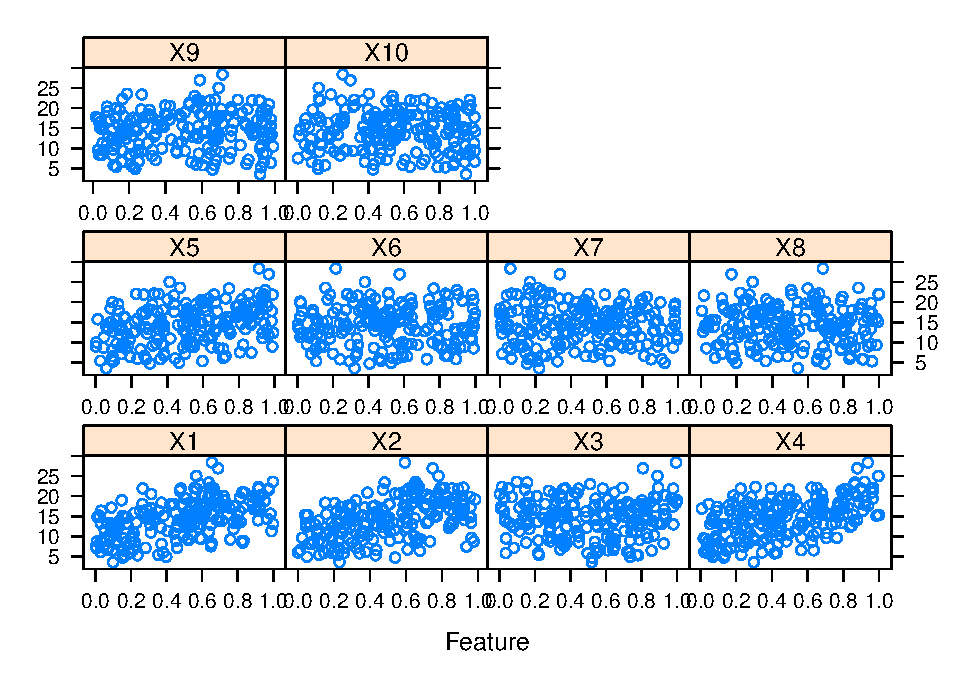
\includegraphics{Weeks-7-8-Homework_files/figure-latex/unnamed-chunk-2-1.pdf}

The plots above show that this data is not stationary as there is some
seasonality in the top of chart. As for the ACF, there is a slow
decrease with lag remaining over the blue lines.

\newpage

\hypertarget{exercise-8.11---3}{%
\section{Exercise 8.11 - 3}\label{exercise-8.11---3}}

For the following series, find an appropriate Box-Cox transformation and
order of differencing in order to obtain stationary data.

\hypertarget{a.-usnetelec}{%
\subsection{\texorpdfstring{a.
\texttt{usnetelec}}{a. usnetelec}}\label{a.-usnetelec}}

\begin{Shaded}
\begin{Highlighting}[]
\KeywordTok{autoplot}\NormalTok{(usnetelec)}
\end{Highlighting}
\end{Shaded}

\includegraphics{Weeks-7-8-Homework_files/figure-latex/unnamed-chunk-3-1.pdf}

\begin{Shaded}
\begin{Highlighting}[]
\KeywordTok{ur.kpss}\NormalTok{(usnetelec) }\OperatorTok\StringTok{ }\KeywordTok{summary}\NormalTok{()}
\end{Highlighting}
\end{Shaded}

\begin{verbatim}
## 
## ####################### 
## # KPSS Unit Root Test # 
## ####################### 
## 
## Test is of type: mu with 3 lags. 
## 
## Value of test-statistic is: 1.464 
## 
## Critical value for a significance level of: 
##                 10pct  5pct 2.5pct  1pct
## critical values 0.347 0.463  0.574 0.739
\end{verbatim}

\begin{Shaded}
\begin{Highlighting}[]
\KeywordTok{ndiffs}\NormalTok{(ibmclose) }\CommentTok{# 1 order of differencing required...non seasonal data}
\end{Highlighting}
\end{Shaded}

\begin{verbatim}
## [1] 1
\end{verbatim}

\begin{Shaded}
\begin{Highlighting}[]
\NormalTok{usnetelec }\OperatorTok\StringTok{ }\KeywordTok{diff}\NormalTok{() }\OperatorTok\StringTok{ }\KeywordTok{autoplot}\NormalTok{()}
\end{Highlighting}
\end{Shaded}

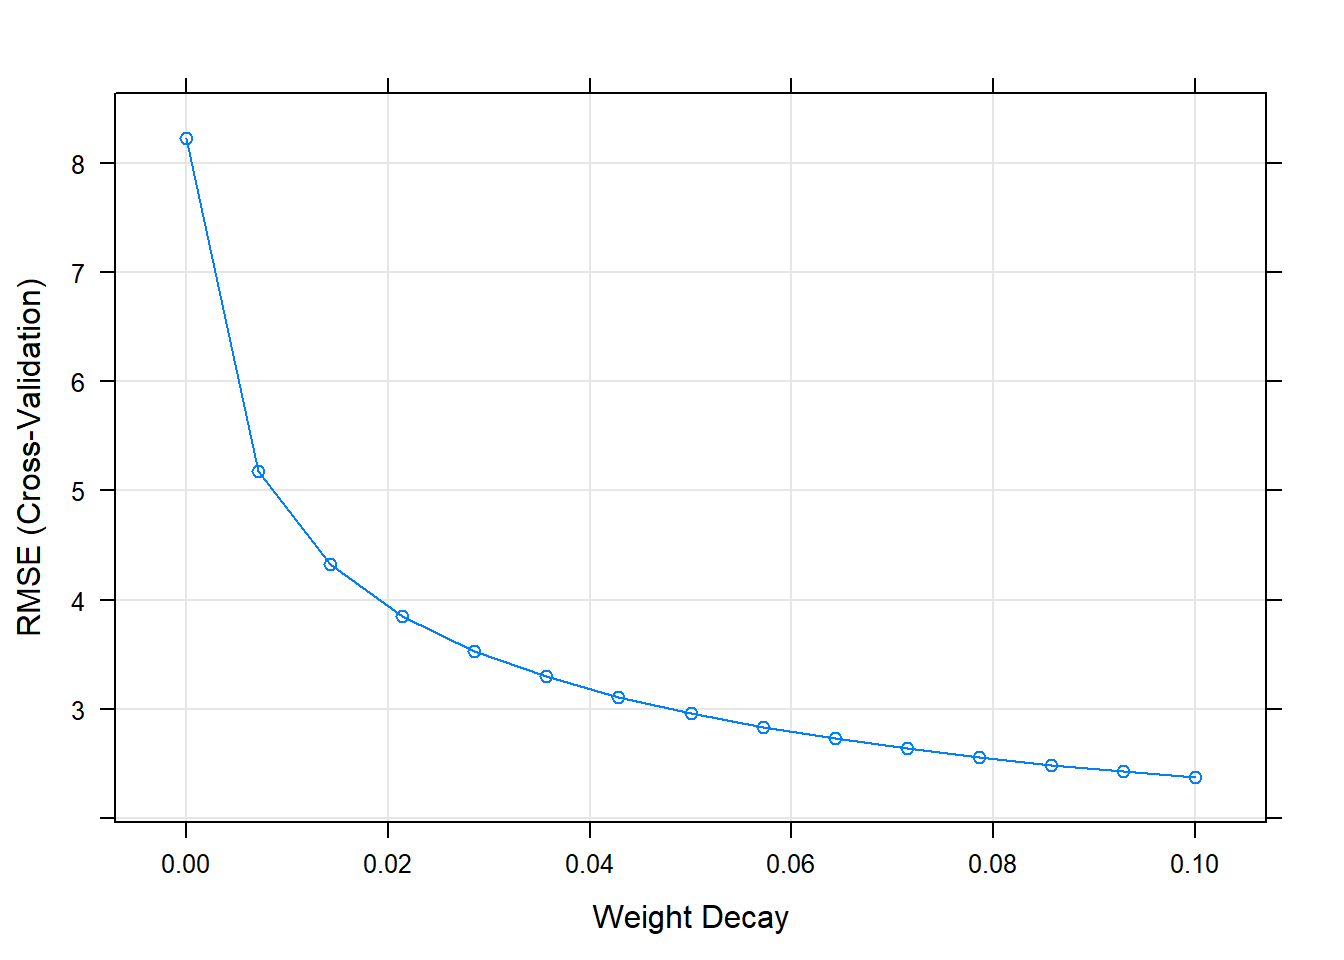
\includegraphics{Weeks-7-8-Homework_files/figure-latex/unnamed-chunk-4-1.pdf}

\hypertarget{b.-usgdp}{%
\subsection{\texorpdfstring{b.
\texttt{usgdp}}{b. usgdp}}\label{b.-usgdp}}

\begin{Shaded}
\begin{Highlighting}[]
\KeywordTok{autoplot}\NormalTok{(usgdp)}
\end{Highlighting}
\end{Shaded}

\includegraphics{Weeks-7-8-Homework_files/figure-latex/unnamed-chunk-5-1.pdf}

\begin{Shaded}
\begin{Highlighting}[]
\KeywordTok{ur.kpss}\NormalTok{(usgdp) }\OperatorTok\StringTok{ }\KeywordTok{summary}\NormalTok{()}
\end{Highlighting}
\end{Shaded}

\begin{verbatim}
## 
## ####################### 
## # KPSS Unit Root Test # 
## ####################### 
## 
## Test is of type: mu with 4 lags. 
## 
## Value of test-statistic is: 4.6556 
## 
## Critical value for a significance level of: 
##                 10pct  5pct 2.5pct  1pct
## critical values 0.347 0.463  0.574 0.739
\end{verbatim}

\begin{Shaded}
\begin{Highlighting}[]
\KeywordTok{ndiffs}\NormalTok{(usgdp)}
\end{Highlighting}
\end{Shaded}

\begin{verbatim}
## [1] 2
\end{verbatim}

\begin{Shaded}
\begin{Highlighting}[]
\KeywordTok{nsdiffs}\NormalTok{(usgdp) }\CommentTok{# no seasonal differencing required}
\end{Highlighting}
\end{Shaded}

\begin{verbatim}
## [1] 0
\end{verbatim}

\begin{Shaded}
\begin{Highlighting}[]
\KeywordTok{autoplot}\NormalTok{(}\KeywordTok{diff}\NormalTok{(}\KeywordTok{diff}\NormalTok{(usgdp)))}
\end{Highlighting}
\end{Shaded}

\includegraphics{Weeks-7-8-Homework_files/figure-latex/unnamed-chunk-6-1.pdf}

\hypertarget{c.-mcopper}{%
\subsection{\texorpdfstring{c.~\texttt{mcopper}}{c.~mcopper}}\label{c.-mcopper}}

\begin{Shaded}
\begin{Highlighting}[]
\KeywordTok{autoplot}\NormalTok{(mcopper)}
\end{Highlighting}
\end{Shaded}

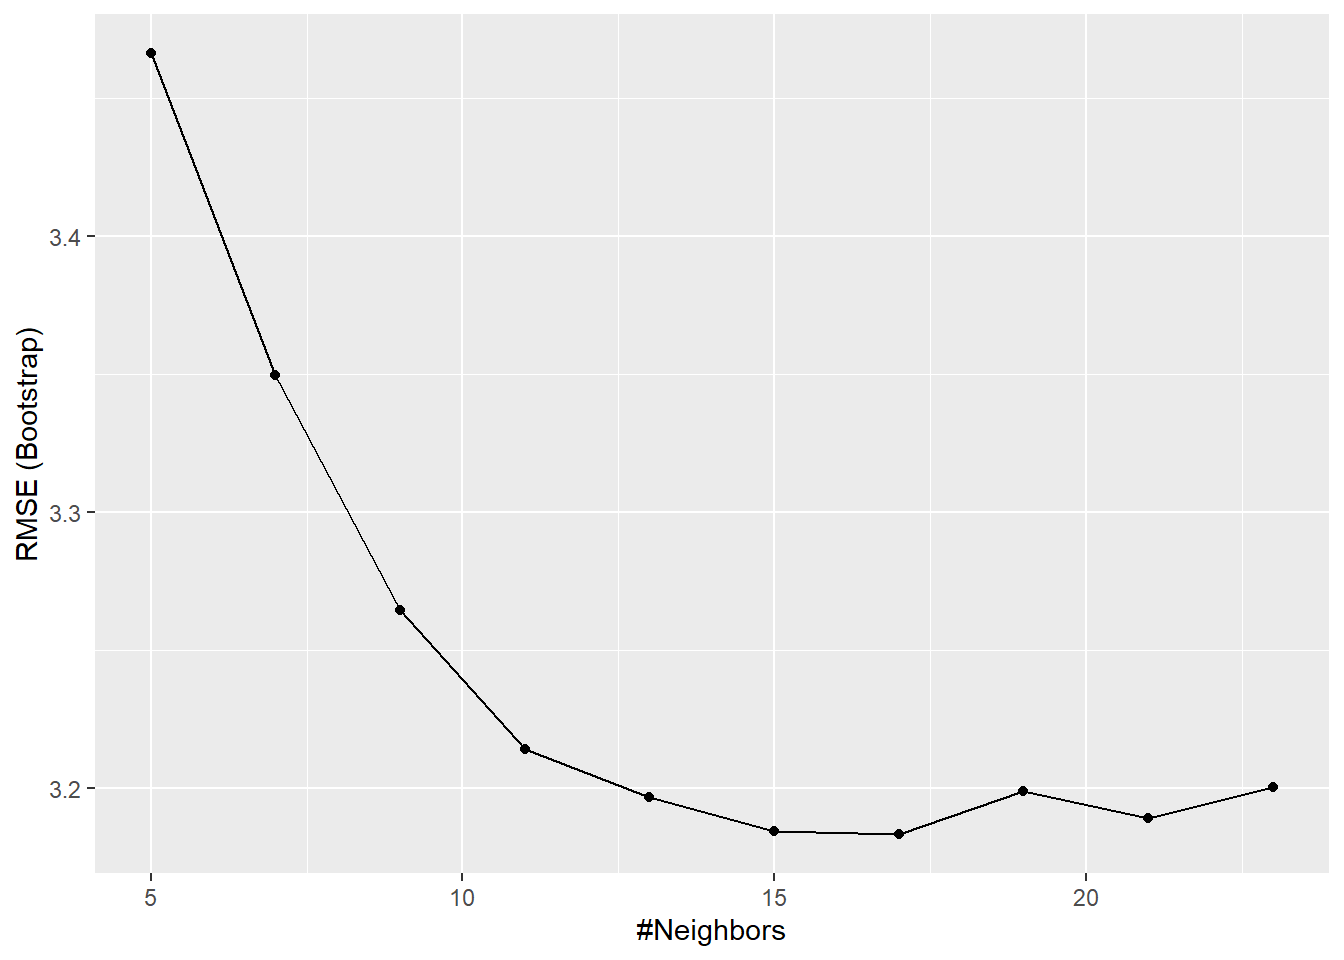
\includegraphics{Weeks-7-8-Homework_files/figure-latex/unnamed-chunk-7-1.pdf}

\begin{Shaded}
\begin{Highlighting}[]
\KeywordTok{ur.kpss}\NormalTok{(mcopper) }\OperatorTok\StringTok{ }\KeywordTok{summary}\NormalTok{()}
\end{Highlighting}
\end{Shaded}

\begin{verbatim}
## 
## ####################### 
## # KPSS Unit Root Test # 
## ####################### 
## 
## Test is of type: mu with 6 lags. 
## 
## Value of test-statistic is: 5.01 
## 
## Critical value for a significance level of: 
##                 10pct  5pct 2.5pct  1pct
## critical values 0.347 0.463  0.574 0.739
\end{verbatim}

\begin{Shaded}
\begin{Highlighting}[]
\KeywordTok{ndiffs}\NormalTok{(mcopper)}
\end{Highlighting}
\end{Shaded}

\begin{verbatim}
## [1] 1
\end{verbatim}

\begin{Shaded}
\begin{Highlighting}[]
\KeywordTok{autoplot}\NormalTok{(}\KeywordTok{diff}\NormalTok{(mcopper))}
\end{Highlighting}
\end{Shaded}

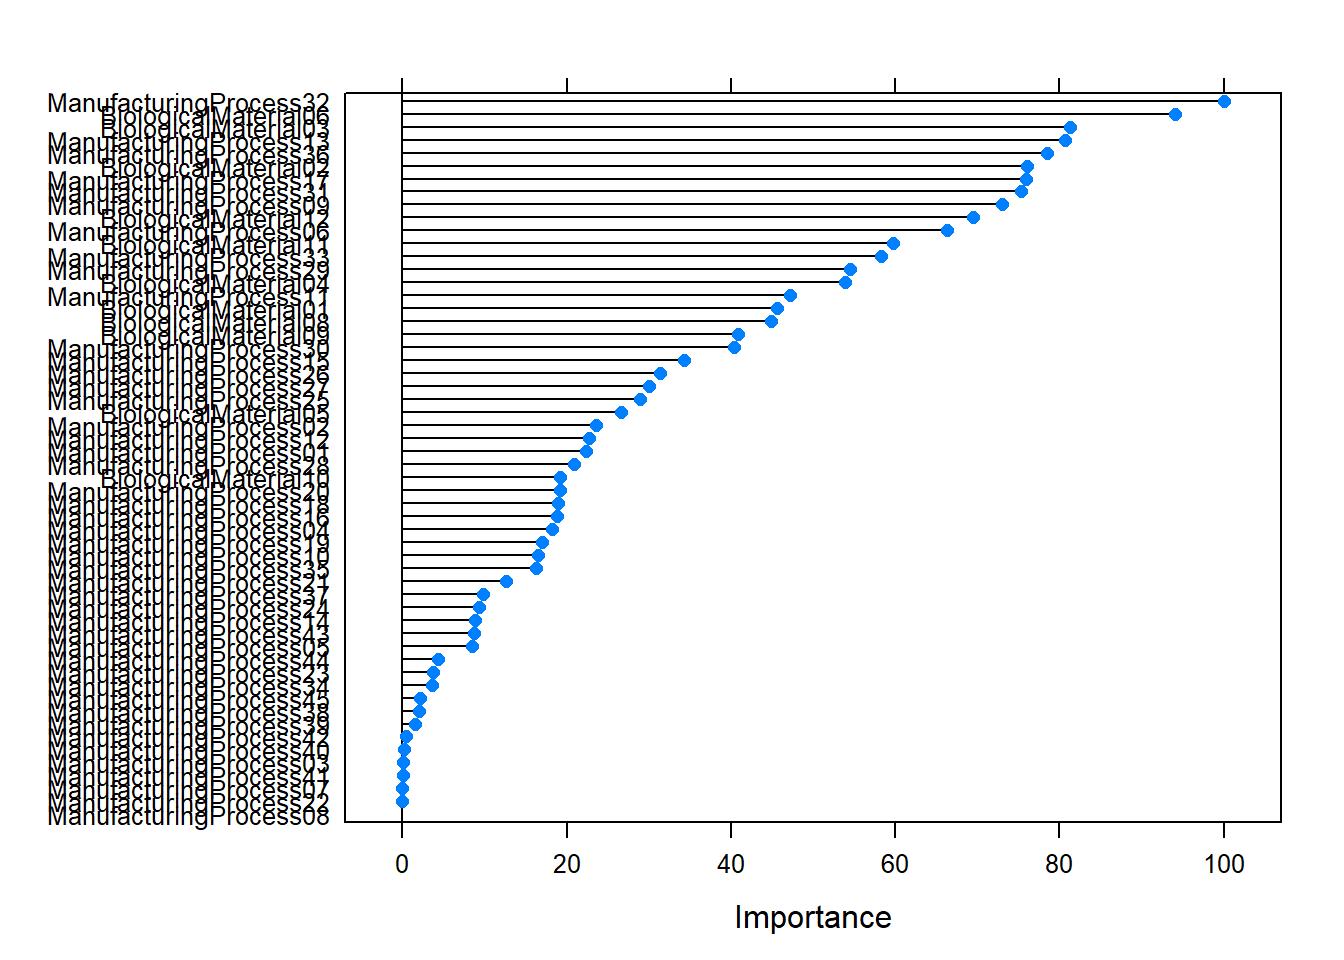
\includegraphics{Weeks-7-8-Homework_files/figure-latex/unnamed-chunk-8-1.pdf}

Let's try transforming the data.

\begin{Shaded}
\begin{Highlighting}[]
\NormalTok{mcopper_lambda <-}\StringTok{ }\KeywordTok{BoxCox.lambda}\NormalTok{(mcopper)}
\NormalTok{mcopper }\OperatorTok\StringTok{ }\KeywordTok{BoxCox}\NormalTok{(mcopper_lambda) }\OperatorTok\StringTok{ }\KeywordTok{diff}\NormalTok{() }\OperatorTok\StringTok{ }\KeywordTok{autoplot}\NormalTok{()}
\end{Highlighting}
\end{Shaded}

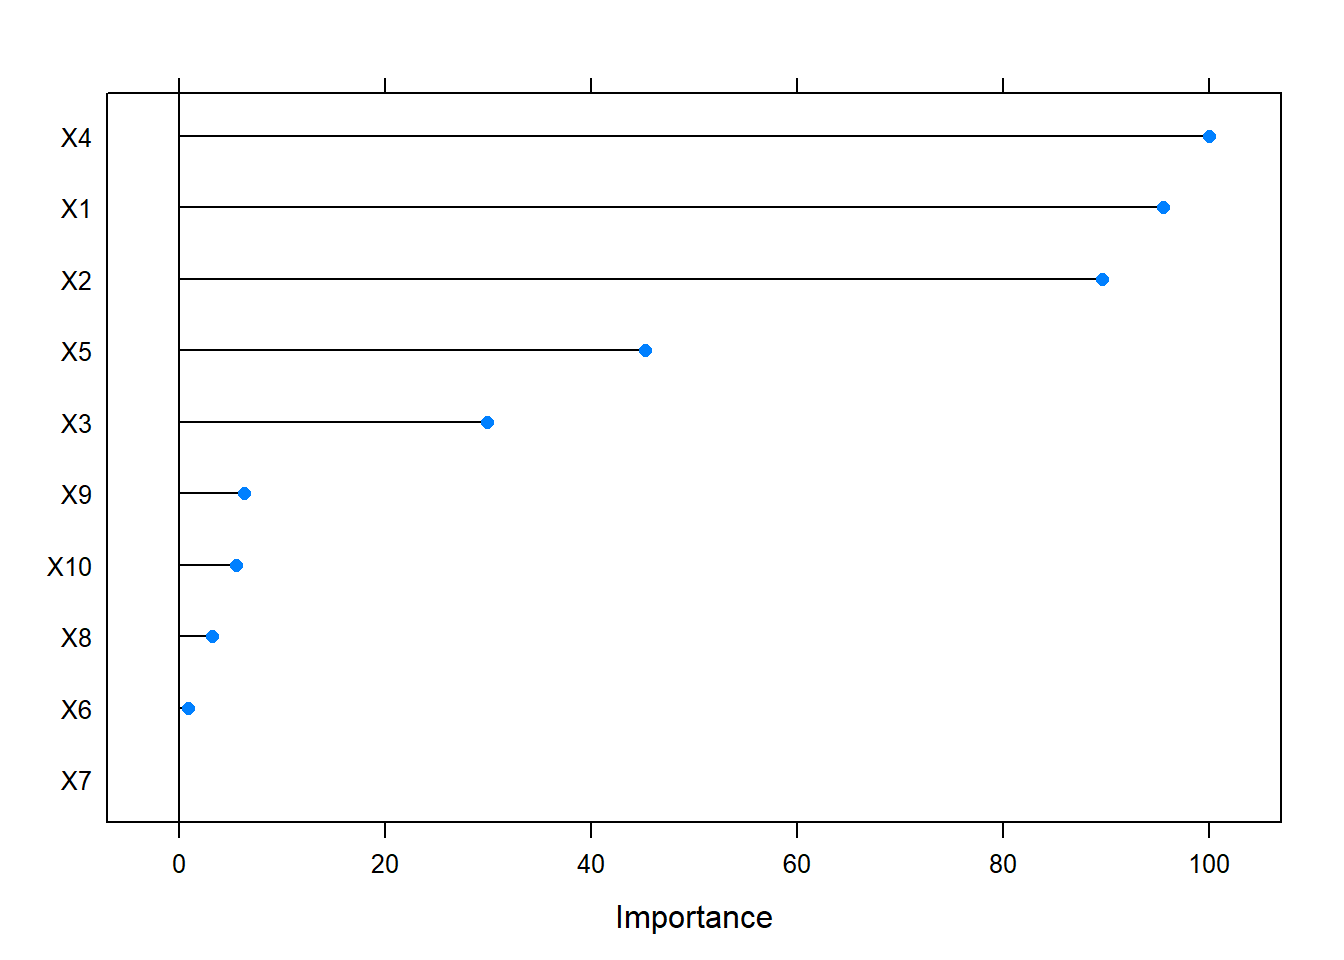
\includegraphics{Weeks-7-8-Homework_files/figure-latex/unnamed-chunk-9-1.pdf}

\hypertarget{d.-enplanements}{%
\subsection{\texorpdfstring{d.~\texttt{enplanements}}{d.~enplanements}}\label{d.-enplanements}}

\begin{Shaded}
\begin{Highlighting}[]
\KeywordTok{autoplot}\NormalTok{(enplanements)}
\end{Highlighting}
\end{Shaded}

\includegraphics{Weeks-7-8-Homework_files/figure-latex/unnamed-chunk-10-1.pdf}

\begin{Shaded}
\begin{Highlighting}[]
\KeywordTok{ur.kpss}\NormalTok{(enplanements) }\OperatorTok\StringTok{ }\KeywordTok{summary}\NormalTok{()}
\end{Highlighting}
\end{Shaded}

\begin{verbatim}
## 
## ####################### 
## # KPSS Unit Root Test # 
## ####################### 
## 
## Test is of type: mu with 5 lags. 
## 
## Value of test-statistic is: 4.4423 
## 
## Critical value for a significance level of: 
##                 10pct  5pct 2.5pct  1pct
## critical values 0.347 0.463  0.574 0.739
\end{verbatim}

\begin{Shaded}
\begin{Highlighting}[]
\KeywordTok{ndiffs}\NormalTok{(enplanements)}
\end{Highlighting}
\end{Shaded}

\begin{verbatim}
## [1] 1
\end{verbatim}

\begin{Shaded}
\begin{Highlighting}[]
\KeywordTok{nsdiffs}\NormalTok{(enplanements)}
\end{Highlighting}
\end{Shaded}

\begin{verbatim}
## [1] 1
\end{verbatim}

Sometimes it is necessary to take both a seasonal difference and a first
difference to obtain stationary data. The second \texttt{diff()} is
seasonal and the first \texttt{diff()} is for first difference.

\begin{Shaded}
\begin{Highlighting}[]
\NormalTok{enp_lambda <-}\StringTok{ }\KeywordTok{BoxCox.lambda}\NormalTok{(enplanements)}
\NormalTok{enplanements }\OperatorTok\StringTok{ }\KeywordTok{BoxCox}\NormalTok{(enp_lambda) }\OperatorTok\StringTok{ }\KeywordTok{diff}\NormalTok{() }\OperatorTok\StringTok{ }\KeywordTok{diff}\NormalTok{() }\OperatorTok\StringTok{ }\KeywordTok{autoplot}\NormalTok{()}
\end{Highlighting}
\end{Shaded}

\includegraphics{Weeks-7-8-Homework_files/figure-latex/unnamed-chunk-11-1.pdf}

\hypertarget{e.-visitors}{%
\subsection{\texorpdfstring{e.
\texttt{visitors}}{e. visitors}}\label{e.-visitors}}

\begin{Shaded}
\begin{Highlighting}[]
\KeywordTok{autoplot}\NormalTok{(visitors)}
\end{Highlighting}
\end{Shaded}

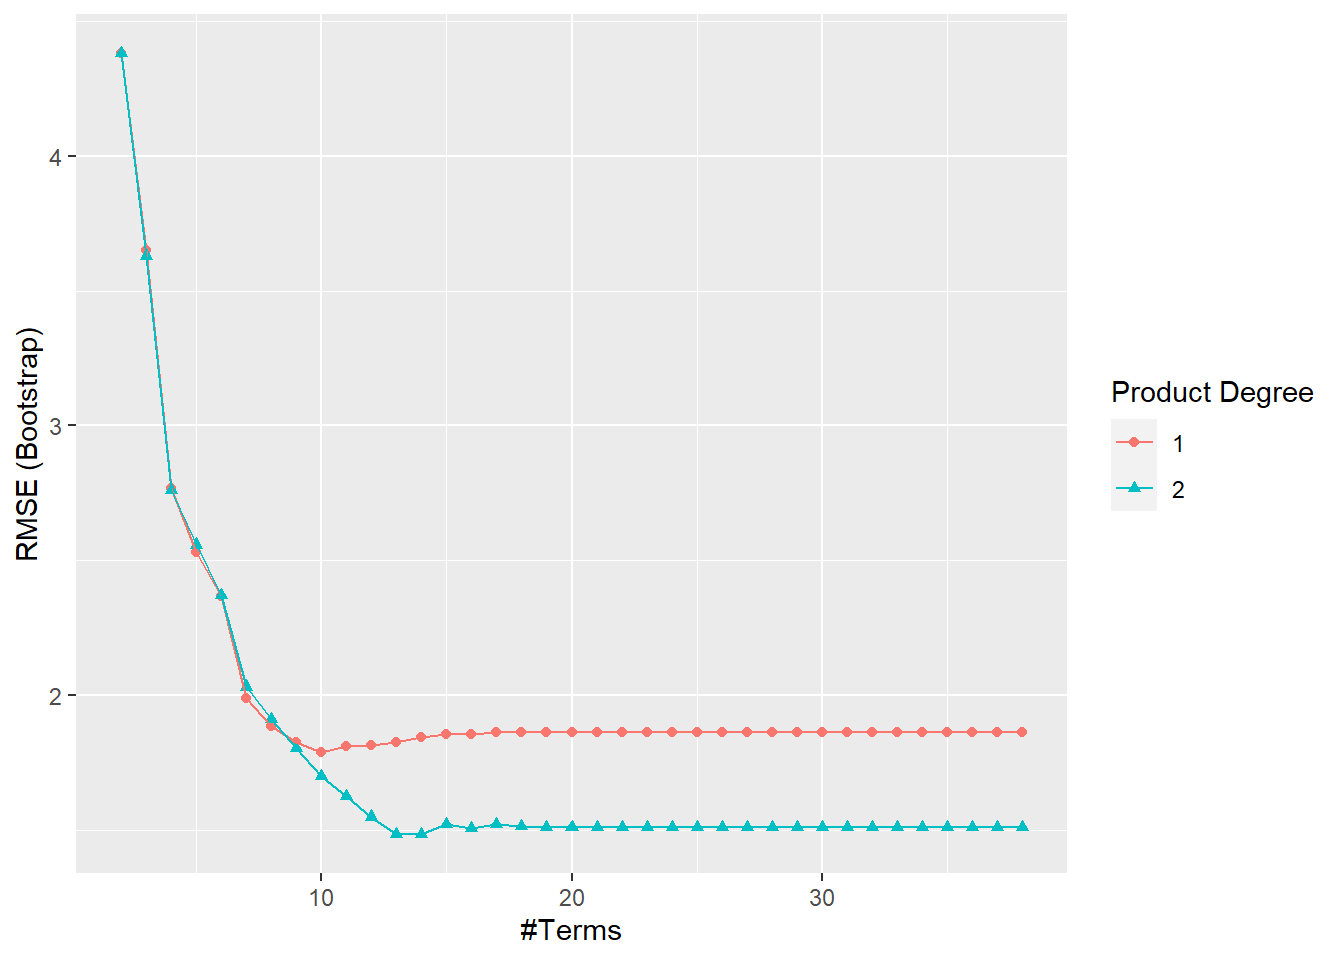
\includegraphics{Weeks-7-8-Homework_files/figure-latex/unnamed-chunk-12-1.pdf}

\begin{Shaded}
\begin{Highlighting}[]
\KeywordTok{ur.kpss}\NormalTok{(visitors) }\OperatorTok\StringTok{ }\KeywordTok{summary}\NormalTok{()}
\end{Highlighting}
\end{Shaded}

\begin{verbatim}
## 
## ####################### 
## # KPSS Unit Root Test # 
## ####################### 
## 
## Test is of type: mu with 4 lags. 
## 
## Value of test-statistic is: 4.6025 
## 
## Critical value for a significance level of: 
##                 10pct  5pct 2.5pct  1pct
## critical values 0.347 0.463  0.574 0.739
\end{verbatim}

\begin{Shaded}
\begin{Highlighting}[]
\KeywordTok{ndiffs}\NormalTok{(visitors)}
\end{Highlighting}
\end{Shaded}

\begin{verbatim}
## [1] 1
\end{verbatim}

\begin{Shaded}
\begin{Highlighting}[]
\KeywordTok{nsdiffs}\NormalTok{(visitors)}
\end{Highlighting}
\end{Shaded}

\begin{verbatim}
## [1] 1
\end{verbatim}

Same situation as with \texttt{enplanements}.

\begin{Shaded}
\begin{Highlighting}[]
\NormalTok{vis_lambda <-}\StringTok{ }\KeywordTok{BoxCox.lambda}\NormalTok{(visitors)}
\NormalTok{visitors }\OperatorTok\StringTok{ }\KeywordTok{BoxCox}\NormalTok{(vis_lambda) }\OperatorTok\StringTok{ }\KeywordTok{diff}\NormalTok{() }\OperatorTok\StringTok{ }\KeywordTok{diff}\NormalTok{() }\OperatorTok\StringTok{ }\KeywordTok{autoplot}\NormalTok{()}
\end{Highlighting}
\end{Shaded}

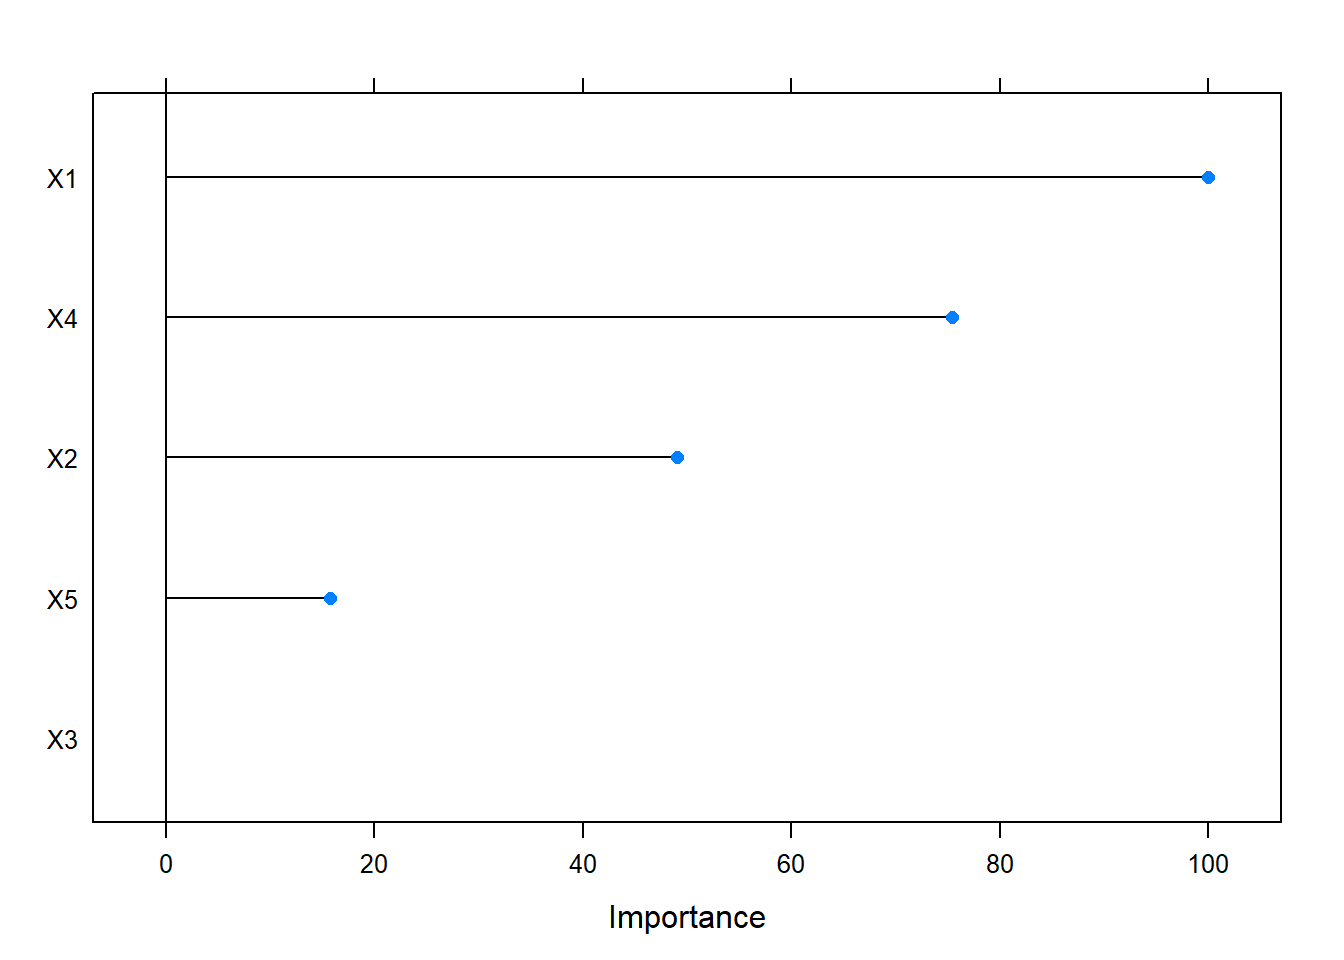
\includegraphics{Weeks-7-8-Homework_files/figure-latex/unnamed-chunk-14-1.pdf}

\newpage

\hypertarget{exercise-8.11---5}{%
\section{Exercise 8.11 - 5}\label{exercise-8.11---5}}

For your retail data (from Exercise 3 in Section 2.10), find the
appropriate order of differencing (after transformation if necessary) to
obtain stationary data.

\begin{Shaded}
\begin{Highlighting}[]
\NormalTok{retaildata <-}\StringTok{ }\NormalTok{readxl}\OperatorTok{::}\KeywordTok{read_excel}\NormalTok{(}\StringTok{"retail.xlsx"}\NormalTok{, }\DataTypeTok{skip=}\DecValTok{1}\NormalTok{)}

\NormalTok{myts <-}\StringTok{ }\KeywordTok{ts}\NormalTok{(retaildata[,}\StringTok{"A3349414R"}\NormalTok{],}
  \DataTypeTok{frequency=}\DecValTok{12}\NormalTok{, }\DataTypeTok{start=}\KeywordTok{c}\NormalTok{(}\DecValTok{1982}\NormalTok{,}\DecValTok{4}\NormalTok{))}

\KeywordTok{autoplot}\NormalTok{(myts)}
\end{Highlighting}
\end{Shaded}

\includegraphics{Weeks-7-8-Homework_files/figure-latex/unnamed-chunk-15-1.pdf}

\begin{Shaded}
\begin{Highlighting}[]
\KeywordTok{ur.kpss}\NormalTok{(myts) }\OperatorTok\StringTok{ }\KeywordTok{summary}\NormalTok{()}
\end{Highlighting}
\end{Shaded}

\begin{verbatim}
## 
## ####################### 
## # KPSS Unit Root Test # 
## ####################### 
## 
## Test is of type: mu with 5 lags. 
## 
## Value of test-statistic is: 5.662 
## 
## Critical value for a significance level of: 
##                 10pct  5pct 2.5pct  1pct
## critical values 0.347 0.463  0.574 0.739
\end{verbatim}

\begin{Shaded}
\begin{Highlighting}[]
\NormalTok{myts_lambda <-}\StringTok{ }\KeywordTok{BoxCox.lambda}\NormalTok{(myts)}
\NormalTok{myts }\OperatorTok\StringTok{ }\KeywordTok{BoxCox}\NormalTok{(}\DataTypeTok{lambda =}\NormalTok{ myts_lambda) }\OperatorTok\StringTok{ }\KeywordTok{ndiffs}\NormalTok{()}
\end{Highlighting}
\end{Shaded}

\begin{verbatim}
## [1] 1
\end{verbatim}

\begin{Shaded}
\begin{Highlighting}[]
\NormalTok{myts }\OperatorTok\StringTok{ }\KeywordTok{BoxCox}\NormalTok{(}\DataTypeTok{lambda =}\NormalTok{ myts_lambda) }\OperatorTok\StringTok{ }\KeywordTok{nsdiffs}\NormalTok{()}
\end{Highlighting}
\end{Shaded}

\begin{verbatim}
## [1] 1
\end{verbatim}

\begin{Shaded}
\begin{Highlighting}[]
\NormalTok{myts }\OperatorTok\StringTok{ }\KeywordTok{BoxCox}\NormalTok{(myts_lambda) }\OperatorTok\StringTok{ }\KeywordTok{diff}\NormalTok{() }\OperatorTok\StringTok{ }\KeywordTok{diff}\NormalTok{() }\OperatorTok\StringTok{ }\KeywordTok{autoplot}\NormalTok{()}
\end{Highlighting}
\end{Shaded}

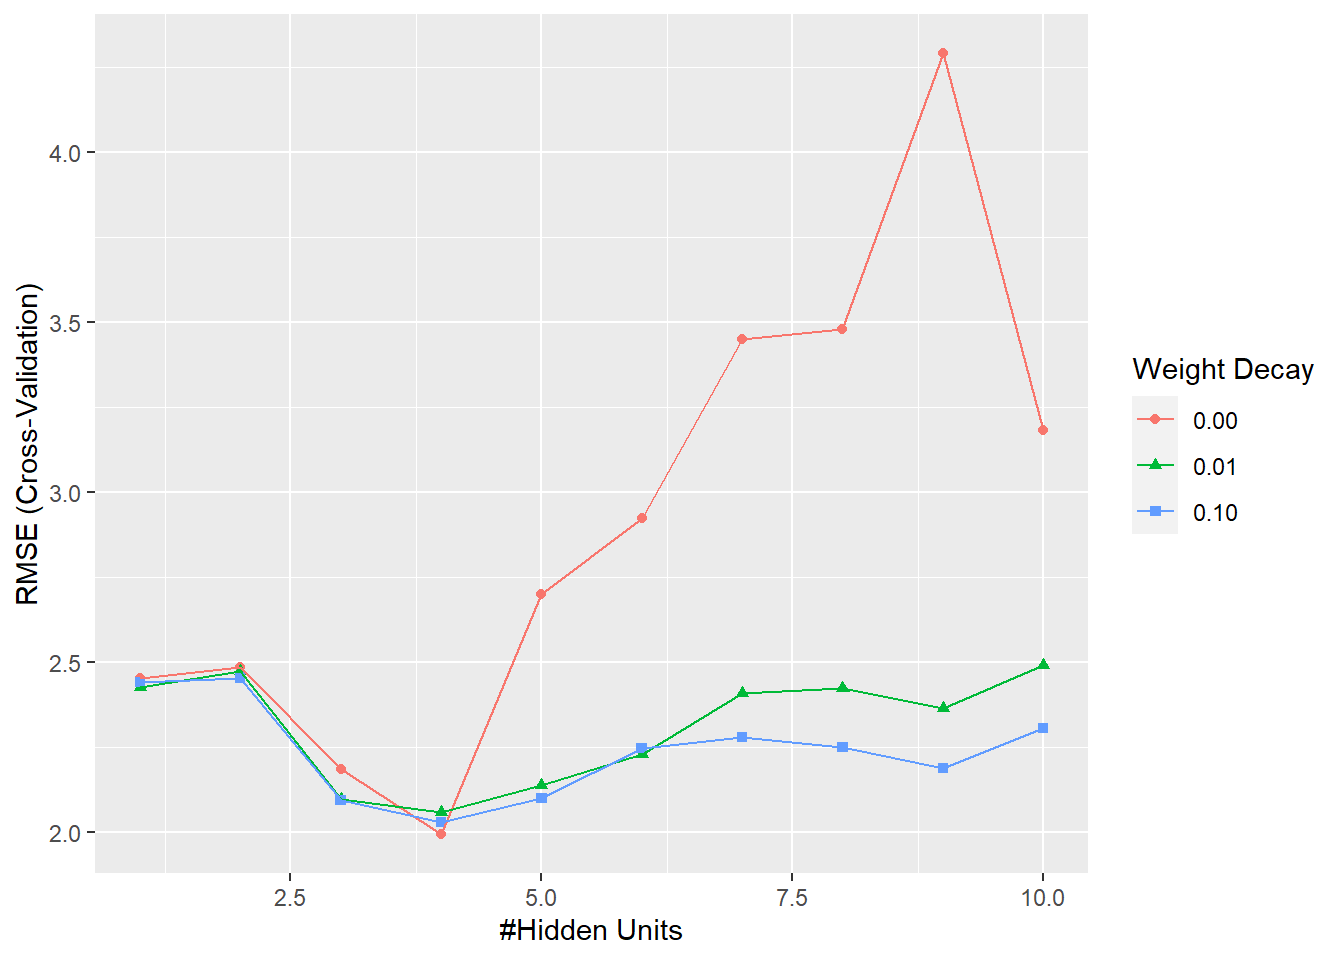
\includegraphics{Weeks-7-8-Homework_files/figure-latex/unnamed-chunk-18-1.pdf}

\newpage

\hypertarget{exercise-8.11---6}{%
\section{Exercise 8.11 - 6}\label{exercise-8.11---6}}

Use R to simulate and plot some data from simple ARIMA models.

\hypertarget{a.-use-the-following-r-code-to-generate-data-from-an-ar1-model-with-1-0.6-and-2-1.-the-process-starts-with-y1-0.}{%
\section{a. Use the following R code to generate data from an AR(1)
model with ϕ1 = 0.6 and σ2 = 1. The process starts with y1 =
0.}\label{a.-use-the-following-r-code-to-generate-data-from-an-ar1-model-with-1-0.6-and-2-1.-the-process-starts-with-y1-0.}}

\begin{Shaded}
\begin{Highlighting}[]
\NormalTok{y <-}\StringTok{ }\KeywordTok{ts}\NormalTok{(}\KeywordTok{numeric}\NormalTok{(}\DecValTok{100}\NormalTok{))}
\NormalTok{e <-}\StringTok{ }\KeywordTok{rnorm}\NormalTok{(}\DecValTok{100}\NormalTok{)}
\ControlFlowTok{for}\NormalTok{(i }\ControlFlowTok{in} \DecValTok{2}\OperatorTok{:}\DecValTok{100}\NormalTok{)}
\NormalTok{  y[i] <-}\StringTok{ }\FloatTok{0.6}\OperatorTok{*}\NormalTok{y[i}\DecValTok{-1}\NormalTok{] }\OperatorTok{+}\StringTok{ }\NormalTok{e[i]}
\end{Highlighting}
\end{Shaded}

\hypertarget{b.-produce-a-time-plot-for-the-series.-how-does-the-plot-change-as-you-change-1}{%
\section{b. Produce a time plot for the series. How does the plot change
as you change
ϕ1?}\label{b.-produce-a-time-plot-for-the-series.-how-does-the-plot-change-as-you-change-1}}

\begin{Shaded}
\begin{Highlighting}[]
\KeywordTok{autoplot}\NormalTok{(y)}
\end{Highlighting}
\end{Shaded}

\includegraphics{Weeks-7-8-Homework_files/figure-latex/unnamed-chunk-20-1.pdf}

\begin{Shaded}
\begin{Highlighting}[]
\NormalTok{y <-}\StringTok{ }\KeywordTok{ts}\NormalTok{(}\KeywordTok{numeric}\NormalTok{(}\DecValTok{100}\NormalTok{))}
\NormalTok{y2 <-}\StringTok{ }\KeywordTok{ts}\NormalTok{(}\KeywordTok{numeric}\NormalTok{(}\DecValTok{100}\NormalTok{))}
\NormalTok{y3 <-}\StringTok{ }\KeywordTok{ts}\NormalTok{(}\KeywordTok{numeric}\NormalTok{(}\DecValTok{100}\NormalTok{))}
\NormalTok{y4 <-}\StringTok{ }\KeywordTok{ts}\NormalTok{(}\KeywordTok{numeric}\NormalTok{(}\DecValTok{100}\NormalTok{))}
\NormalTok{e <-}\StringTok{ }\KeywordTok{rnorm}\NormalTok{(}\DecValTok{100}\NormalTok{)}
\ControlFlowTok{for}\NormalTok{(i }\ControlFlowTok{in} \DecValTok{2}\OperatorTok{:}\DecValTok{100}\NormalTok{)\{}
\NormalTok{  y[i] <-}\StringTok{ }\FloatTok{0.6}\OperatorTok{*}\NormalTok{y[i}\DecValTok{-1}\NormalTok{] }\OperatorTok{+}\StringTok{ }\NormalTok{e[i]}
\NormalTok{  y2[i] <-}\StringTok{ }\FloatTok{0.1}\OperatorTok{*}\NormalTok{y2[i}\DecValTok{-1}\NormalTok{] }\OperatorTok{+}\StringTok{ }\NormalTok{e[i]}
\NormalTok{  y3[i] <-}\StringTok{ }\FloatTok{0.8}\OperatorTok{*}\NormalTok{y3[i}\DecValTok{-1}\NormalTok{] }\OperatorTok{+}\StringTok{ }\NormalTok{e[i]}
\NormalTok{  y4[i] <-}\StringTok{ }\DecValTok{1}\OperatorTok{*}\NormalTok{y4[i}\DecValTok{-1}\NormalTok{] }\OperatorTok{+}\StringTok{ }\NormalTok{e[i]}
\NormalTok{\}}
\NormalTok{gridExtra}\OperatorTok{::}\KeywordTok{grid.arrange}\NormalTok{(}
  \KeywordTok{autoplot}\NormalTok{(y2) }\OperatorTok{+}\StringTok{ }\KeywordTok{ggtitle}\NormalTok{(}\StringTok{"phi = 0.1"}\NormalTok{),}
  \KeywordTok{autoplot}\NormalTok{(y) }\OperatorTok{+}\StringTok{ }\KeywordTok{ggtitle}\NormalTok{(}\StringTok{"phi = 0.6"}\NormalTok{),}
  \KeywordTok{autoplot}\NormalTok{(y3) }\OperatorTok{+}\StringTok{ }\KeywordTok{ggtitle}\NormalTok{(}\StringTok{"phi = 0.8"}\NormalTok{),}
  \KeywordTok{autoplot}\NormalTok{(y4) }\OperatorTok{+}\StringTok{ }\KeywordTok{ggtitle}\NormalTok{(}\StringTok{"phi = 1"}\NormalTok{), }\DataTypeTok{nrow =} \DecValTok{2}
\NormalTok{)}
\end{Highlighting}
\end{Shaded}

\includegraphics{Weeks-7-8-Homework_files/figure-latex/unnamed-chunk-21-1.pdf}

\hypertarget{c.-write-your-own-code-to-generate-data-from-an-ma1-model-with-1-0.6-and-2-1.}{%
\subsection{c.~Write your own code to generate data from an MA(1) model
with θ1 = 0.6 and σ2 =
1.}\label{c.-write-your-own-code-to-generate-data-from-an-ma1-model-with-1-0.6-and-2-1.}}

\begin{Shaded}
\begin{Highlighting}[]
\NormalTok{y_ma1 <-}\StringTok{ }\KeywordTok{ts}\NormalTok{(}\KeywordTok{numeric}\NormalTok{(}\DecValTok{100}\NormalTok{))}
\NormalTok{e <-}\StringTok{ }\KeywordTok{rnorm}\NormalTok{(}\DecValTok{100}\NormalTok{)}
\ControlFlowTok{for}\NormalTok{(i }\ControlFlowTok{in} \DecValTok{2}\OperatorTok{:}\DecValTok{100}\NormalTok{)}
\NormalTok{  y_ma1[i] <-}\StringTok{ }\FloatTok{0.6}\OperatorTok{*}\NormalTok{e[i}\DecValTok{-1}\NormalTok{] }\OperatorTok{+}\StringTok{ }\NormalTok{e[i]}
\end{Highlighting}
\end{Shaded}

\hypertarget{d.-produce-a-time-plot-for-the-series.-how-does-the-plot-change-as-you-change-1}{%
\subsection{d.~Produce a time plot for the series. How does the plot
change as you change
θ1?}\label{d.-produce-a-time-plot-for-the-series.-how-does-the-plot-change-as-you-change-1}}

\begin{Shaded}
\begin{Highlighting}[]
\KeywordTok{autoplot}\NormalTok{(y_ma1)}
\end{Highlighting}
\end{Shaded}

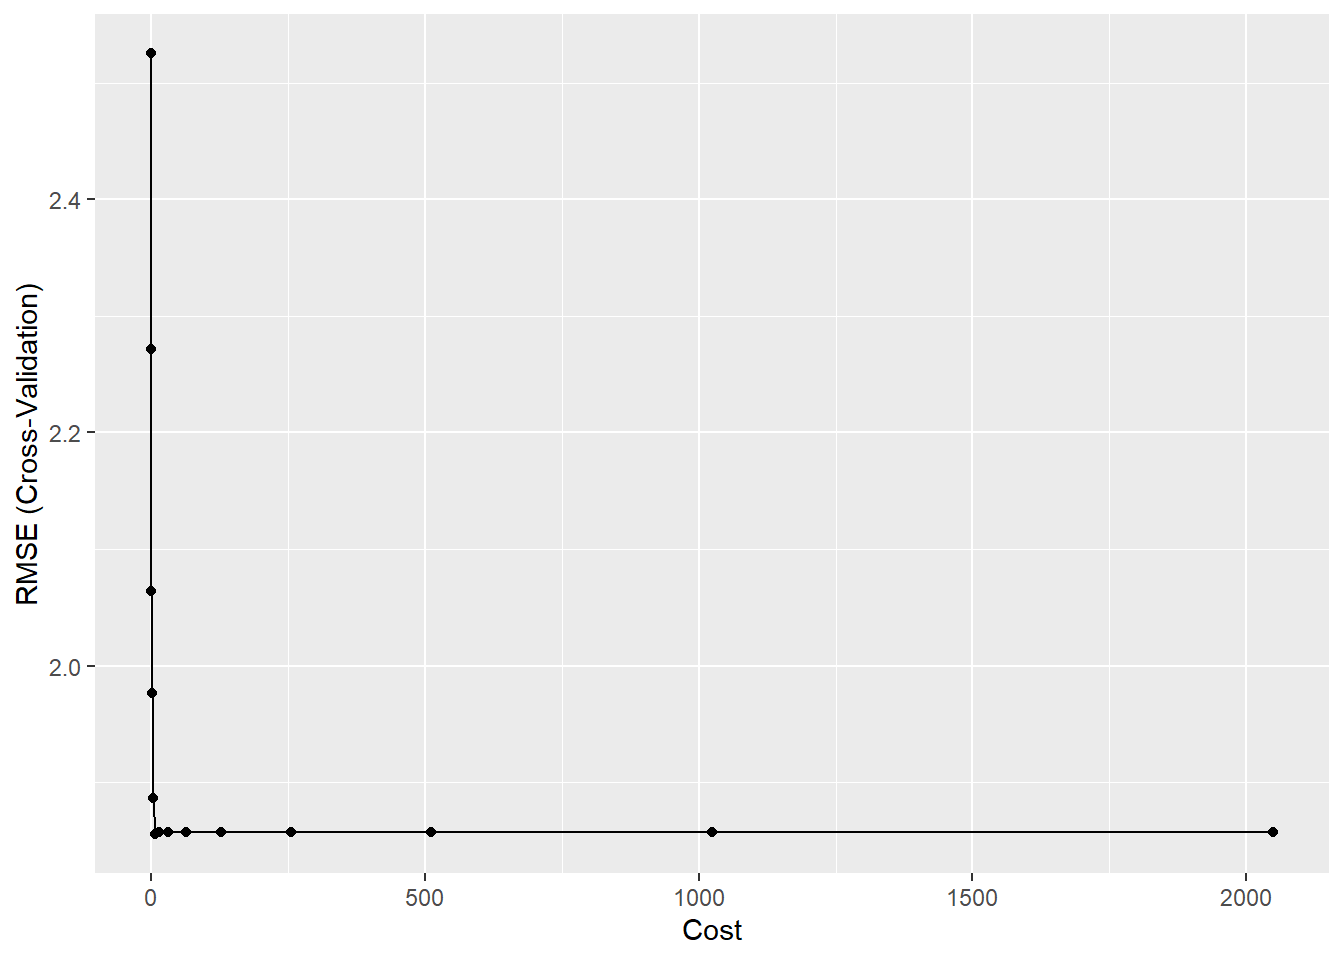
\includegraphics{Weeks-7-8-Homework_files/figure-latex/unnamed-chunk-23-1.pdf}

\begin{Shaded}
\begin{Highlighting}[]
\NormalTok{y_ma1 <-}\StringTok{ }\KeywordTok{ts}\NormalTok{(}\KeywordTok{numeric}\NormalTok{(}\DecValTok{100}\NormalTok{))}
\NormalTok{y2_ma1 <-}\StringTok{ }\KeywordTok{ts}\NormalTok{(}\KeywordTok{numeric}\NormalTok{(}\DecValTok{100}\NormalTok{))}
\NormalTok{y3_ma1 <-}\StringTok{ }\KeywordTok{ts}\NormalTok{(}\KeywordTok{numeric}\NormalTok{(}\DecValTok{100}\NormalTok{))}
\NormalTok{y4_ma1 <-}\StringTok{ }\KeywordTok{ts}\NormalTok{(}\KeywordTok{numeric}\NormalTok{(}\DecValTok{100}\NormalTok{))}
\NormalTok{e <-}\StringTok{ }\KeywordTok{rnorm}\NormalTok{(}\DecValTok{100}\NormalTok{)}
\ControlFlowTok{for}\NormalTok{(i }\ControlFlowTok{in} \DecValTok{2}\OperatorTok{:}\DecValTok{100}\NormalTok{)\{}
\NormalTok{  y_ma1[i] <-}\StringTok{ }\FloatTok{0.6}\OperatorTok{*}\NormalTok{e[i}\DecValTok{-1}\NormalTok{] }\OperatorTok{+}\StringTok{ }\NormalTok{e[i]}
\NormalTok{  y2_ma1[i] <-}\StringTok{ }\FloatTok{0.1}\OperatorTok{*}\NormalTok{e[i}\DecValTok{-1}\NormalTok{] }\OperatorTok{+}\StringTok{ }\NormalTok{e[i]}
\NormalTok{  y3_ma1[i] <-}\StringTok{ }\FloatTok{0.8}\OperatorTok{*}\NormalTok{e[i}\DecValTok{-1}\NormalTok{] }\OperatorTok{+}\StringTok{ }\NormalTok{e[i]}
\NormalTok{  y4_ma1[i] <-}\StringTok{ }\DecValTok{1}\OperatorTok{*}\NormalTok{e[i}\DecValTok{-1}\NormalTok{] }\OperatorTok{+}\StringTok{ }\NormalTok{e[i]}
\NormalTok{\}}
\NormalTok{gridExtra}\OperatorTok{::}\KeywordTok{grid.arrange}\NormalTok{(}
  \KeywordTok{autoplot}\NormalTok{(y2_ma1) }\OperatorTok{+}\StringTok{ }\KeywordTok{ggtitle}\NormalTok{(}\StringTok{"phi = 0.1"}\NormalTok{),}
  \KeywordTok{autoplot}\NormalTok{(y_ma1) }\OperatorTok{+}\StringTok{ }\KeywordTok{ggtitle}\NormalTok{(}\StringTok{"phi = 0.6"}\NormalTok{),}
  \KeywordTok{autoplot}\NormalTok{(y3_ma1) }\OperatorTok{+}\StringTok{ }\KeywordTok{ggtitle}\NormalTok{(}\StringTok{"phi = 0.8"}\NormalTok{),}
  \KeywordTok{autoplot}\NormalTok{(y4_ma1) }\OperatorTok{+}\StringTok{ }\KeywordTok{ggtitle}\NormalTok{(}\StringTok{"phi = 1"}\NormalTok{), }\DataTypeTok{nrow =} \DecValTok{2}
\NormalTok{)}
\end{Highlighting}
\end{Shaded}

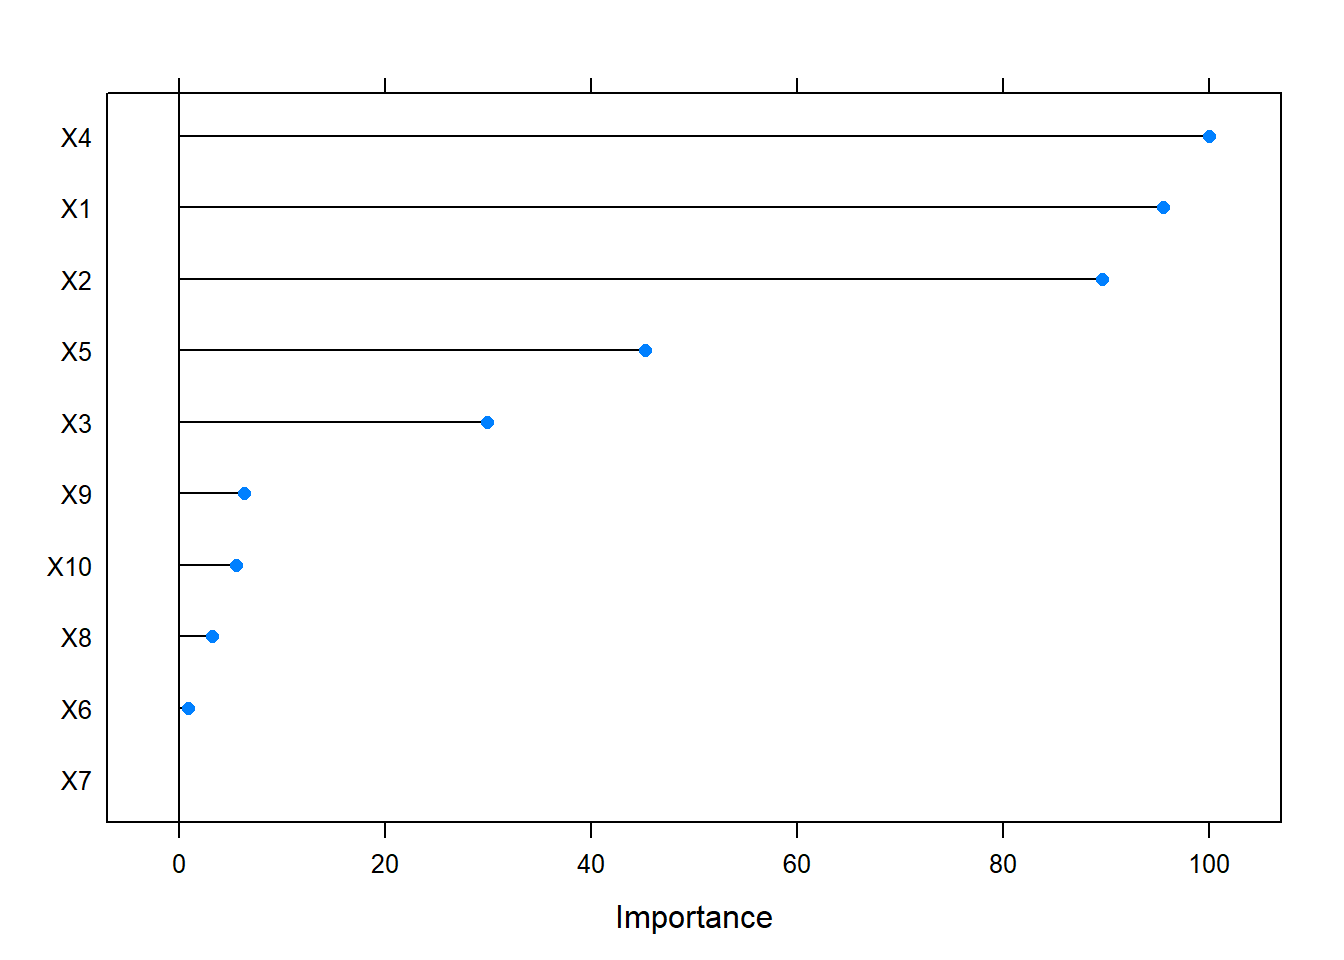
\includegraphics{Weeks-7-8-Homework_files/figure-latex/unnamed-chunk-24-1.pdf}

\hypertarget{e.-generate-data-from-an-arma11-model-with-1-0.6-1-0.6-and-2-1.}{%
\subsection{e. Generate data from an ARMA(1,1) model with ϕ1 = 0.6, θ1 =
0.6 and σ2 =
1.}\label{e.-generate-data-from-an-arma11-model-with-1-0.6-1-0.6-and-2-1.}}

\begin{Shaded}
\begin{Highlighting}[]
\NormalTok{y_ARMA <-}\StringTok{ }\KeywordTok{ts}\NormalTok{(}\KeywordTok{numeric}\NormalTok{(}\DecValTok{100}\NormalTok{))}
\NormalTok{e <-}\StringTok{ }\KeywordTok{rnorm}\NormalTok{(}\DecValTok{100}\NormalTok{)}
\ControlFlowTok{for}\NormalTok{(i }\ControlFlowTok{in} \DecValTok{2}\OperatorTok{:}\DecValTok{100}\NormalTok{)}
\NormalTok{  y_ARMA[i] <-}\StringTok{ }\FloatTok{0.6}\OperatorTok{*}\NormalTok{y_ARMA[i}\DecValTok{-1}\NormalTok{] }\OperatorTok{+}\StringTok{ }\FloatTok{0.6}\OperatorTok{*}\NormalTok{e[i}\DecValTok{-1}\NormalTok{] }\OperatorTok{+}\StringTok{ }\NormalTok{e[i]}
\end{Highlighting}
\end{Shaded}

\hypertarget{f.-generate-data-from-an-ar2-model-with-1-0.8-2-0.3-and-2-1.-note-that-these-parameters-will-give-a-non-stationary-series.}{%
\subsection{f.~Generate data from an AR(2) model with ϕ1 = −0.8, ϕ2 =
0.3 and σ2 = 1. (Note that these parameters will give a non-stationary
series.)}\label{f.-generate-data-from-an-ar2-model-with-1-0.8-2-0.3-and-2-1.-note-that-these-parameters-will-give-a-non-stationary-series.}}

\begin{Shaded}
\begin{Highlighting}[]
\NormalTok{y_AR2 <-}\StringTok{ }\KeywordTok{ts}\NormalTok{(}\KeywordTok{numeric}\NormalTok{(}\DecValTok{100}\NormalTok{))}
\NormalTok{e <-}\StringTok{ }\KeywordTok{rnorm}\NormalTok{(}\DecValTok{100}\NormalTok{)}
\ControlFlowTok{for}\NormalTok{(i }\ControlFlowTok{in} \DecValTok{3}\OperatorTok{:}\DecValTok{100}\NormalTok{)}
\NormalTok{  y_AR2[i] <-}\StringTok{ }\NormalTok{(}\OperatorTok{-}\FloatTok{0.8}\OperatorTok{*}\NormalTok{y_AR2[i}\DecValTok{-1}\NormalTok{]) }\OperatorTok{+}\StringTok{ }\NormalTok{(}\FloatTok{0.3}\OperatorTok{*}\NormalTok{y_AR2[i}\DecValTok{-2}\NormalTok{]) }\OperatorTok{+}\StringTok{ }\NormalTok{e[i]}
\end{Highlighting}
\end{Shaded}

\hypertarget{g.graph-the-latter-two-series-and-compare-them.}{%
\subsection{g.Graph the latter two series and compare
them.}\label{g.graph-the-latter-two-series-and-compare-them.}}

\begin{Shaded}
\begin{Highlighting}[]
\NormalTok{gridExtra}\OperatorTok{::}\KeywordTok{grid.arrange}\NormalTok{(}\KeywordTok{autoplot}\NormalTok{(y_ARMA) }\OperatorTok{+}\StringTok{ }\KeywordTok{ggtitle}\NormalTok{(}\StringTok{"ARMA"}\NormalTok{), }\KeywordTok{autoplot}\NormalTok{(y_AR2) }\OperatorTok{+}\StringTok{ }\KeywordTok{ggtitle}\NormalTok{(}\StringTok{"AR(2)"}\NormalTok{))}
\end{Highlighting}
\end{Shaded}

\includegraphics{Weeks-7-8-Homework_files/figure-latex/unnamed-chunk-27-1.pdf}

\newpage

\hypertarget{exercise-8.11---7}{%
\section{Exercise 8.11 - 7}\label{exercise-8.11---7}}

Consider \texttt{wmurders}, the number of women murdered each year (per
100,000 standard population) in the United States.

\hypertarget{a.-by-studying-appropriate-graphs-of-the-series-in-r-find-an-appropriate-arimapdq-model-for-these-data.}{%
\subsection{a. By studying appropriate graphs of the series in R, find
an appropriate ARIMA(p,d,q) model for these
data.}\label{a.-by-studying-appropriate-graphs-of-the-series-in-r-find-an-appropriate-arimapdq-model-for-these-data.}}

\begin{Shaded}
\begin{Highlighting}[]
\KeywordTok{autoplot}\NormalTok{(wmurders)}
\end{Highlighting}
\end{Shaded}

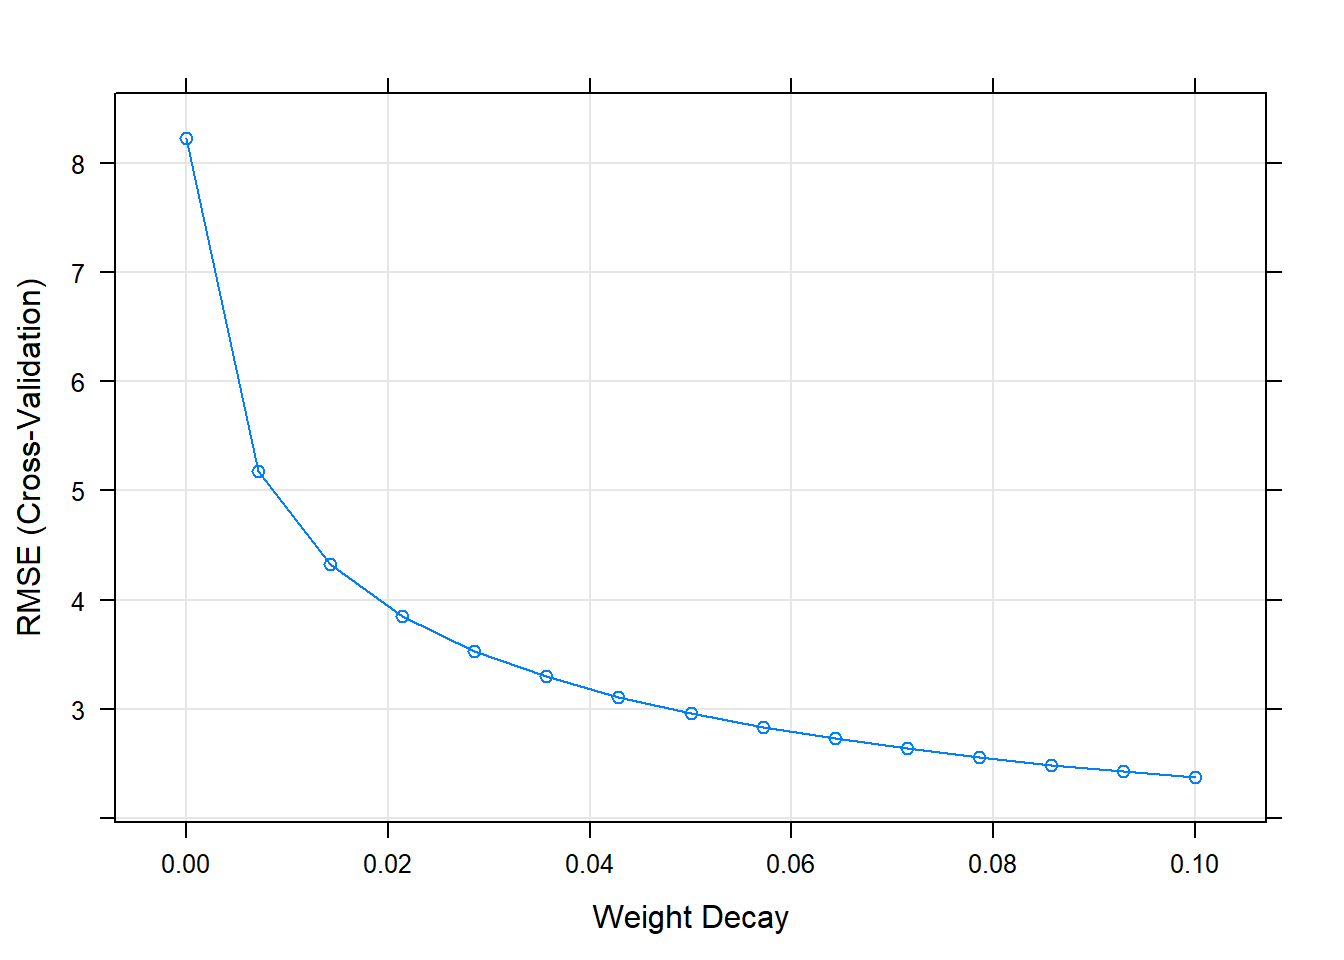
\includegraphics{Weeks-7-8-Homework_files/figure-latex/unnamed-chunk-28-1.pdf}

\begin{Shaded}
\begin{Highlighting}[]
\KeywordTok{ndiffs}\NormalTok{(wmurders)}
\end{Highlighting}
\end{Shaded}

\begin{verbatim}
## [1] 2
\end{verbatim}

\begin{Shaded}
\begin{Highlighting}[]
\NormalTok{wm_lambda <-}\StringTok{ }\KeywordTok{BoxCox.lambda}\NormalTok{(wmurders)}
\NormalTok{wmurders }\OperatorTok\StringTok{ }\KeywordTok{BoxCox}\NormalTok{(wm_lambda) }\OperatorTok\StringTok{ }\KeywordTok{diff}\NormalTok{() }\OperatorTok\StringTok{ }\KeywordTok{diff}\NormalTok{()  }\OperatorTok\StringTok{ }\KeywordTok{ggtsdisplay}\NormalTok{()}
\end{Highlighting}
\end{Shaded}

\includegraphics{Weeks-7-8-Homework_files/figure-latex/unnamed-chunk-28-2.pdf}

\begin{Shaded}
\begin{Highlighting}[]
\NormalTok{wm_fit <-}\StringTok{ }\KeywordTok{Arima}\NormalTok{(wmurders, }\DataTypeTok{order =} \KeywordTok{c}\NormalTok{(}\DecValTok{1}\NormalTok{,}\DecValTok{2}\NormalTok{,}\DecValTok{1}\NormalTok{)) }
\KeywordTok{summary}\NormalTok{(wm_fit)}
\end{Highlighting}
\end{Shaded}

\begin{verbatim}
## Series: wmurders 
## ARIMA(1,2,1) 
## 
## Coefficients:
##           ar1      ma1
##       -0.2434  -0.8261
## s.e.   0.1553   0.1143
## 
## sigma^2 estimated as 0.04632:  log likelihood=6.44
## AIC=-6.88   AICc=-6.39   BIC=-0.97
## 
## Training set error measures:
##                       ME      RMSE       MAE        MPE     MAPE      MASE
## Training set -0.01065956 0.2072523 0.1528734 -0.2149476 4.335214 0.9400996
##                    ACF1
## Training set 0.02176343
\end{verbatim}

\hypertarget{b.-should-you-include-a-constant-in-the-model-explain.}{%
\subsection{b. Should you include a constant in the model?
Explain.}\label{b.-should-you-include-a-constant-in-the-model-explain.}}

In the chapter, it stated that we should not include a constant if the d
= 2, so we will not include a constant here.

\hypertarget{c.-write-this-model-in-terms-of-the-backshift-operator.}{%
\subsection{c.~Write this model in terms of the backshift
operator.}\label{c.-write-this-model-in-terms-of-the-backshift-operator.}}

\hypertarget{d.-fit-the-model-using-r-and-examine-the-residuals.-is-the-model-satisfactory}{%
\subsection{d.~Fit the model using R and examine the residuals. Is the
model
satisfactory?}\label{d.-fit-the-model-using-r-and-examine-the-residuals.-is-the-model-satisfactory}}

\begin{Shaded}
\begin{Highlighting}[]
\KeywordTok{checkresiduals}\NormalTok{(wm_fit)}
\end{Highlighting}
\end{Shaded}

\includegraphics{Weeks-7-8-Homework_files/figure-latex/unnamed-chunk-30-1.pdf}

\begin{verbatim}
## 
##  Ljung-Box test
## 
## data:  Residuals from ARIMA(1,2,1)
## Q* = 12.419, df = 8, p-value = 0.1335
## 
## Model df: 2.   Total lags used: 10
\end{verbatim}

This model is satisfactory because we see all autocorrelations within
the blue lines showing that the residuals are acting like the white
noise.

\hypertarget{e.-forecast-three-times-ahead.-check-your-forecasts-by-hand-to-make-sure-that-you-know-how-they-have-been-calculated.}{%
\subsection{e. Forecast three times ahead. Check your forecasts by hand
to make sure that you know how they have been
calculated.}\label{e.-forecast-three-times-ahead.-check-your-forecasts-by-hand-to-make-sure-that-you-know-how-they-have-been-calculated.}}

\begin{Shaded}
\begin{Highlighting}[]
\KeywordTok{forecast}\NormalTok{(wm_fit, }\DataTypeTok{h=}\DecValTok{3}\NormalTok{)}
\end{Highlighting}
\end{Shaded}

\begin{verbatim}
##      Point Forecast    Lo 80    Hi 80    Lo 95    Hi 95
## 2005       2.470660 2.194836 2.746484 2.048824 2.892496
## 2006       2.363106 1.986351 2.739862 1.786908 2.939304
## 2007       2.252833 1.765391 2.740276 1.507354 2.998313
\end{verbatim}

\hypertarget{f.-create-a-plot-of-the-series-with-forecasts-and-prediction-intervals-for-the-next-three-periods-shown.}{%
\subsection{f.~Create a plot of the series with forecasts and prediction
intervals for the next three periods
shown.}\label{f.-create-a-plot-of-the-series-with-forecasts-and-prediction-intervals-for-the-next-three-periods-shown.}}

\begin{Shaded}
\begin{Highlighting}[]
\KeywordTok{autoplot}\NormalTok{(}\KeywordTok{forecast}\NormalTok{(wm_fit, }\DataTypeTok{h=}\DecValTok{3}\NormalTok{), }\DataTypeTok{PI =}\NormalTok{ T)}
\end{Highlighting}
\end{Shaded}

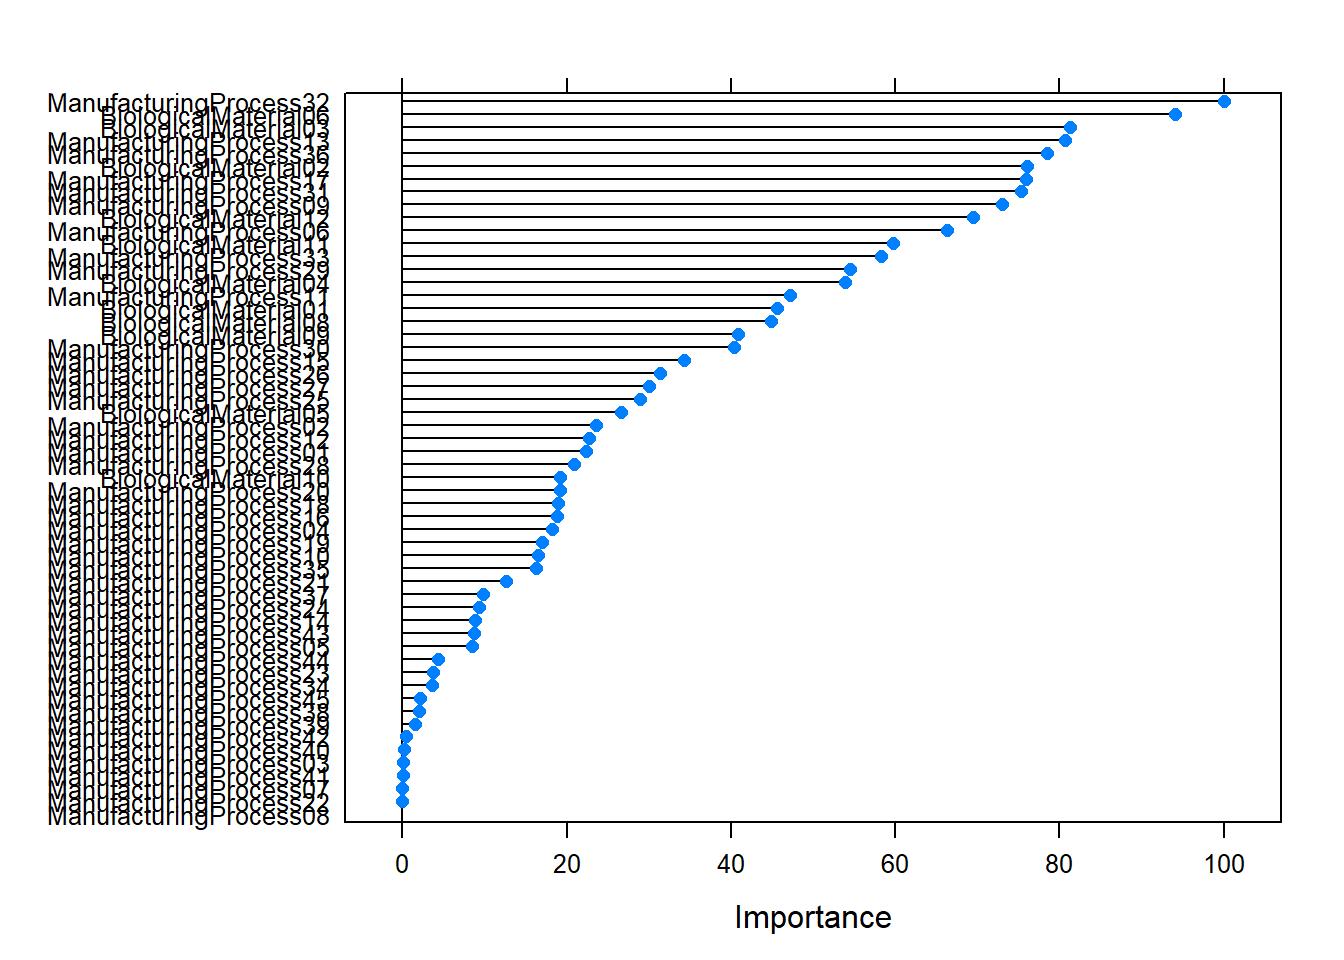
\includegraphics{Weeks-7-8-Homework_files/figure-latex/unnamed-chunk-32-1.pdf}

\hypertarget{g.-does-auto.arima-give-the-same-model-you-have-chosen-if-not-which-model-do-you-think-is-better}{%
\subsection{g. Does auto.arima() give the same model you have chosen? If
not, which model do you think is
better?}\label{g.-does-auto.arima-give-the-same-model-you-have-chosen-if-not-which-model-do-you-think-is-better}}

\begin{Shaded}
\begin{Highlighting}[]
\NormalTok{wm_fit2 <-}\StringTok{ }\KeywordTok{auto.arima}\NormalTok{(wmurders)}
\KeywordTok{summary}\NormalTok{(wm_fit2)}
\end{Highlighting}
\end{Shaded}

\begin{verbatim}
## Series: wmurders 
## ARIMA(1,2,1) 
## 
## Coefficients:
##           ar1      ma1
##       -0.2434  -0.8261
## s.e.   0.1553   0.1143
## 
## sigma^2 estimated as 0.04632:  log likelihood=6.44
## AIC=-6.88   AICc=-6.39   BIC=-0.97
## 
## Training set error measures:
##                       ME      RMSE       MAE        MPE     MAPE      MASE
## Training set -0.01065956 0.2072523 0.1528734 -0.2149476 4.335214 0.9400996
##                    ACF1
## Training set 0.02176343
\end{verbatim}

The \texttt{auto.arima()} function does give us the same model.


\end{document}
